% !TEX root = ferguson-dissertation.tex

\chapter{Interacting with \sys}
\label{sec:messages}

We now expand upon the three message types introduced
in the overview: requests, queries, and hints. Table~\ref{tab:concepts}
has a concise specification of these messages, and their
relation to other key concepts in \sys.

%Shares and the share tree do not affect the network
%themselves. Instead, \sys maintains a second data-structure, the
%\emph{policy tree}, which determines network-wide policy.  \sys
%ensures two key invariants. First, it ensures that the policy tree
%always has the same tree-structure as the share tree. Second, it
%ensures that all \emph{policy atoms} in a policy tree node are authorized by
%the corresponding share.
%
%Each node in the policy tree holds a set of policy atoms, which we write
%as follows:
%\[
%  \paneprin{user}{host}{app}:\{F\}\rightarrow\panemsg
%\]
%A policy atom indicates that a principal affects a flowgroup in the
%manner determined by \panemsg, which we describe below.

\section{Requests}
\label{sec:Requests}

A \emph{request} affects the state of the network for some interval of time. 
%{\color{red} When \sys receives a request, it first checks that the principal
%has the necessary privileges in the share tree. Second, it checks if
%the request can co-exist with previously accepted requests by checking
%the policy tree for the start and end times, as we will describe in
%\Cref{sec:PolicyTrees}. }
%
By default, requests take effect immediately and do not expire;
specific start and end times may optionally be provided.  Verifying if
a request can be granted may require walking the tree's hierarchy,
depending on the type of request.  This design allows resources to be
oversubscribed; overallocation is prevented when requests are granted,
and not when shares are created.

Participatory networks may support requests for a variety of network
resources and services, which we detail next.

\tightparagraph{Access Control}
The simplest type of network service exposed by \sys is access control
-- the ability to allow and deny traffic, using the \textbf{Allow} and
\textbf{Deny} requests.  Like all requests, they specify a flowgroup
describing the affected traffic, and the share which the principal is
using to invoke the privilege.
Each access control privilege is optionally constrained by a specified
number of seconds, $n$.
To exceed this limit, principals must periodically renew requests.
Shares lacking the ability to allow or deny traffic have $n = 0$.
When creating a sub-share, a principal cannot exceed these constraints. For example,
if a share carries the privilege to \priv{Deny} traffic for up to
300 seconds, a sub-share cannot be created with the privilege to \priv{Deny}
traffic for up to 301 seconds; similarly, a sub-share could not be created
with the privilege to \priv{Allow} traffic.

The handling of a given packet is ultimately decided by the
composition of every matching access control request. This composition
makes use of the share tree's hierarchy to resolve conflicts -- for
example, an access control request made on a child share overrides
those in parent shares.  We defer further discussion of \sys's general
approach to conflict resolution until
\Cref{sec:conflicts}.

With each request, the principal can specify a fulfillment mode, either
\emph{strict} or \emph{partial}. These are provided for atomicity and
convenience. In strict mode, \sys rejects a request if it would be
(partially) overridden by any previous request.
%optional example
For example, if a user wants to allow connections to TCP ports
1000-2000, but there exists a request in a sub-share that denies port
1024, \sys rejects the request, explaining why.  In partial mode, \sys
implements the request, and informs the user that it was only
partially satisfied;
%optional example
in the same example, \sys would inform the user that it has allowed
ports 1000-1023, and 1025-2000.

These modes exist for two reasons: first, to avoid race conditions in
request allocations, and second, to avoid complicated, fine-grained
specifications that depend on \sys's current state. We defer a more
complete discussion of the strict and partial fulfillment modes until
\Cref{sec:strict-partial}.

\begin{figure}[t]
\centering
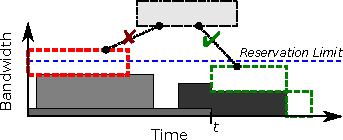
\includegraphics[width=0.6\textwidth]{figs/sched}
\caption{Example user request for reserved bandwidth;
\sys determines that it cannot be fulfilled until time $t$.}
\label{fig:sched}
\end{figure}


\tightparagraph{Guaranteed Minimum Bandwidth}
\sys also provides a \priv{Reserve} privilege which provides
guaranteed minimum bandwidth (GMB) between two hosts.
Shares which contain the privilege to reserve bandwidth are limited
by a modified token bucket:
it has the usual attributes of fill rate $F$, capacity $C$, and maximum
drain rate $M$, and an additional minimum drain rate $m$. This lower
bound prevents reservations with very low drain rates that could
last indefinitely. A simple reservation with maximum
bandwidth $B$ is a special case with $F = M = B; C = m = 0$. GMB
reservations are ultimately implemented by \sys's runtime as a
sequence of forwarding actions and switch queues, as we describe in
\Cref{sec:FullSystem}. Requests which cannot be implemented are
rejected.

Figure~\ref{fig:sched} shows a simple example in which a principal
has requested an immediate bandwidth reservation. \sys determines
that granting the request will exceed the share's available bandwidth.
The principal then examines the share's schedule of available bandwidth
and sends a new request for a reservation
to start at $t$; \sys accepts the request and later implements it.

When creating sub-shares of shares with GMB privileges, the sub-share's
token bucket must ``fit inside'' the parent's token bucket; parents cannot
provide more tokens to their children than they receive. However, a share's
tokens can be over-subscribed by its sub-shares. When a request is granted,
it draws tokens from all of its parent shares, up to the root of the tree, thus
preventing over-allocation.

\tightparagraph{Path Control}
A third request type directs flows through or around middleboxes using
\priv{Waypoint} and \priv{Avoid}.
For example, a university's network administrators can
route students' traffic through a packet shaper during business hours,
and security researchers can avoid intrusion detection systems for traffic to be collected by honeypots.
Shares contain sets of IP addresses listing the middleboxes which
they can route through or avoid, and, as with flowgroups, sub-shares may
only contain subsets of their parents' sets.
\sys implements \priv{Waypoint} and \priv{Avoid} by installing flow-specific
forwarding rules along a path determined by
fixing or deleting nodes as appropriate when routing over the network graph
(\Cref{sec:NIB}). Requests to create unrealizable paths are rejected.

\tightparagraph{Rate-limits}
\sys supports rate-limit requests which result in matching traffic 
being routed through
ports with established rate-limiters, as available in current switches.
While basic, such requests can be used to mitigate DOS attacks or
enforce traffic contracts between tenants in a shared datacenter.
\sys's global view of the network enables it to make best use of the switches'
features and place rate-limiters close to the traffic's source, as we describe in \Cref{sec:NIB}.
Like \sys's bandwidth reservations, rate-limits are currently restricted to circuits;
a network with distributed rate-limiters, such as those proposed
by Raghavan, \etal~\cite{Raghavan:2007}, could support more general limits.
Their integration is left as future work.

\section{Queries}
\label{sec:Queries}

\sys also supports messages to query the state of the network.
These queries may be for general information about the network,
such as the type of a link (\eg, copper or optical), the set of hosts
located downstream of a particular port, or other properties.
Each share may contain a list of properties which it is privileged
to read. This list is similar to a ``view'' on a database; when sub-shares
are created, this view may be further occluded. While these restrictions
provide basic privacy protection when exposing the network's state,
they are not complete. For example, if a switch has three links, and
a principal has the privilege to read the sending and receiving rates
on two of the links, but not the third, it can infer the rate on the third link.
We leave a more complete development of privacy protections as
future work.

The current OpenFlow specifications and design make a number of
properties available which principals in \sys may query including:
 the number (or list) of hosts behind a particular
port, port-specific diagnostic data such as the number of packets
dropped, the number of CRC errors, etc., the physical and topological
location of switches, and the access medium of links. In the future,
we would like to support additional details we believe would
benefit applications such as the current signal-to-noise ratio or
broadcasting power of wireless access points.

\sys also supports a ``network weather service'' which provides coarse
information about current traffic conditions. For example, statistics
about the total amount of traffic over a core link are available, but
not statistics about individual flows. By integrating \sys with a
project like Frenetic~\cite{Foster:2010}, we expect it could support
the ability to query the traffic statistics of individual flows, as
such queries require a more robust OpenFlow runtime than our current
implementation.

Applications can issue queries to the \sys controller to improve the
user experience. For example, Hadoop could use the weather service to
place reducers away from currently-congested parts of the network, and
streaming video players can determine that a wireless access point is
attached to a cellular modem or similarly constrained backhaul as
Shieh, \etal proposed~\cite{Shieh11netquery}.

\section{Hints}
\label{sec:Hints}

The final type of message in \sys is a hint. Hints are used to provide
the network with information which may improve the application's or
network's performance, without creating an additional
requirement. Providing hints across abstraction boundaries is a
natural feature in other systems.
For example, if a three-tier web application makes
a request to the database layer, and hints to the caching layer that it
won't make the same request again in the near future, the cache may
choose to skip storing the result.

Three hints which are useful for networked applications include: the
size (in bytes) of a flow, a desired flow-completion deadline, and the
predictability of future traffic. \sys can use flow size information
to spread large flows across multiple paths of equal-cost, as in Mahout~\cite{curtis11mahout} or
Hedera~\cite{alfares10hedera}.  Deadlines
can be communicated to supporting routers such as those proposed in
D3~\cite{wilson11d3}. And hints about traffic predictability can be
used by traffic optimizers such MicroTE~\cite{Benson2011microte}.

\sys \emph{may} use hints to derive and install policy atoms which affect
related traffic, although it gives no guarantee or notification to the user. 
For example, a hint that a flow is short may generate
a policy atom to increase that flow's priority. We call such hints
\emph{realized}, and their corresponding policy atoms are tagged as
merely hints (\cf Table~\ref{tab:concepts}).

The integration of hints, which can benefit non-\sys systems, as in
the examples above, is deliberate. \sys provides a network
administrator with the framework to delegate privileges, divide
resources, and account for their usage; the ability to issue hints is
a privilege, particularly those which affect limited resources.  The
framework provided by \sys makes it more feasible to implement hints
in an untrusted environment, where malicious principals may issue
false or excessive hints in an attempt to gain an advantage.

Finally, in the absence of transactional-style requests (\eg, a
request for ``resource A \emph{or} resource B''), \sys's hints are a
more flexible way to provide information to the network than via
requests. In this use, hints share a similar role to \sys's partial
fulfillment mode for requests (\Cref{sec:strict-partial}).

\begin{comment}
Hints are not promises, and can always be ignored by the \sys controller. The 
two best examples we have so far are:
\begin{enumerate}
\item ``This is an RPC'' -- it will be short and should have low-latency.
\item ``Size of flow'' hint -- this came up in our discussion with Scott Shenker,
where it would be useful for queues in a switch or spreading elephants across
multiple links.
\item ``Predictable traffic'' hint -- useful for something like Theo's MicroTE~\cite{Benson2011microte}
\end{enumerate}
\end{comment}

\begin{landscape}
\begin{table*}
\centering 
\begin{small}
\[
\begin{array}{ll@{\,}c@{\,}ll}
\hline
\textrm{Share} & S & \in & 
%
\{P\} \times \{F\} \times \{ \panepriv \} & 
%
  \textrm{A share gives principals some privileges to
    affect a set of flows.} \\
%
\textrm{Principal} & P & \mathord{::=} &
%
\paneprin{\textrm{user}}{\textrm{host}}{\textrm{app}} &
% 
  \textrm{A triple consisting of an \emph{application}, running on a
    \emph{host} by a \emph{user}.} \\
%
\textrm{Flow} & F & \mathord{::=} & \langle\textbf{srcIP}\mathord{=}n_1,\textbf{dstIP}\mathord{=}n_2, &
%
  \textrm{A set of packets with shared properties: source and destination IP address,} \\
%
& & & \quad\textbf{proto}\mathord{=}n_3,\textbf{srcPort}\mathord{=}n_4,\textbf{dstPort}\mathord{=}n_5\rangle &
%
  \qquad\textrm{transport protocol, and source and destination transport ports.}\\
%
\textrm{Privilege} & \panepriv & ::= &
%
\textbf{CanDeny}~n \mid \textbf{CanAllow}~n &
%
\textrm{The privileges to allow or deny traffic for up to $n$ seconds (optional).} \\
%
& & & \mid \textbf{CanReserve}~n \mid \textbf{CanRateLimit}~n & 
%
  \textrm{The privileges to reserve bandwidth or set rate-limits, up to
    $n$ MB.} \\
 %
& & & \mid \textbf{CanWaypoint}~\{\textit{IP}\}\mid \textbf{CanAvoid}~\{\textit{IP}\} & 
%
  \textrm{The privileges to direct traffic through or around particular IP addresses.} \\
\hline
%
\textrm{Message} & \textit{Msg} & \mathord{::=} &
%
P:\{F\} : S \rightarrow ( \panereq~\panetspec \mid \panehint~\panetspec \mid \panequery) &
%
\textrm{A message from a principal with a request, hint, or query using a share.} \\
%
\textrm{Time Spec} & \panetspec & ::= & \textbf{from}~t_1~\textbf{until}~t_2 &
%
\textrm{An optional specification from time $t_1$ until $t_2$.} \\
%
\textrm{Request} & \panereq & \mathord{::=} & 
%
\textbf{Allow} \mid \textbf{Deny} &
%
\textrm{Request to allow/deny traffic.}
\\
%
& & &  \mid \textbf{Reserve}~n \mid \textbf{RateLimit}~n~ &
%
  \textrm{Request to reserve $n$ MB or rate-limit to $n$ MB.} \\
%
& & & \mid \textbf{Waypoint}~\textit{IP} \mid \textbf{Avoid}~\textit{IP} &
%
\textrm{Waypoint/avoid traffic through a middlebox with the given IP address.} \\
%
\textrm{Query} & \panequery & \mathord{::=} &
%
\textbf{TrafficBetween}~\textit{srcIP}~\textit{dstIP} \mid ... &
%
\textrm{Query the total traffic between two hosts.} \\
%
\textrm{Hint} & \panehint & \mathord{::=} &
%
\textbf{Duration}~t \mid ... & \textrm{Hint that the flow's duration is $t$.} \\
%
\textrm{Policy Atom} & \panepolatom & \mathord{::=} & 
%
P:\{F\} \rightarrow \panereq~\panetspec &
%
\textrm{A requested modification of network state.} \\
%
& & \mid & \textbf{Hint}~P:\{F\} \rightarrow
\panereq~\panetspec &
%
\textrm{A realized hint; it may be removed if it conflicts with a future request.} \\
\hline
\end{array}
\]
\end{small}
\caption{Main concepts in \sys}  \vspace{-1em}
\label{tab:concepts}
\end{table*}

\end{landscape}

\chapter{The Two Challenges}
\label{sec:two-challenges}

Participatory networking faces two key challenges to its realization.
The first is how to safely decompose control and visibility of the network,
and the second is how to resolve conflicts between participants and across requests.
We now explain how \sys's design overcomes these challenges.

\section{Privilege Delegation}
\label{sec:delegation}

\begin{figure}[t]
\centering
\subfigure[]{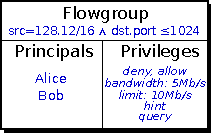
\includegraphics[width=0.35\textwidth]{figs/share}}\hfill
\subfigure[]{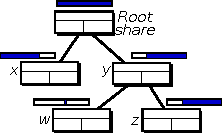
\includegraphics[width=0.35\textwidth]{figs/sharehierarchy}}
\caption{(a) A \sys share. (b) A share
hierarchy. The rectangle above each share represents a flowgroup
according to one dimension (\eg, source IP). Sub-shares are defined
on a subset of their parent's flowgroup, and may not have more permissive
privileges than their parent.}
\label{fig:shares}
\end{figure}

%\vskip 1em

This section presents the semantics of shares and how principals'
messages are authorized in more detail. The \sys
controller maintains two key data structures. First, the \emph{share
  tree} determines the privileges that principals have to read or write
  network state. The tree-structure allows principals to create new shares and
delegate authority to each other. The share tree itself does not
affect the state of the network. Instead, the second key
data-structure, the \emph{policy tree}, holds \emph{policy atoms} that
can affect the network. \sys maintains the invariant that all policy
atoms in the policy tree are properly authorized by the share tree at
all times.

%\section{Share Tree\label{sec:sharetree}}
\vskip 1em

A share-tree is an $n$-ary tree of \emph{shares}, where a share gives
a set of \emph{principals} some \emph{privileges} to affect a set
of \emph{flows} in the network. We elaborate on these terms below.

\tightparagraph{Principals}
A \sys principal is a triple consisting of an application running on a
host by a user. A principal may be
\paneprin{Skype}{192.168.1.7}{Alice} or
\paneprin{Hadoop}{10.20.20.20}{Bob} for example. Shares in \sys are held by
principal-sets.  We abbreviate singleton sets to their principal. We
also use wildcards to denote large sets. \eg, \paneprinuser{Alice} is
the set of all principals with Alice as the user, and
\paneprinapp{Hadoop} is the set of all principals with Hadoop as the
application. We write \paneprinall \ to denote the set of all
principals.

Principals send messages to the \sys controller to request resources
and query the state of the network. For example, the principal
\paneprin{Skype}{192.168.1.7}{Alice} may request low-latency service
between the Skype call's source and destination, and the principal
\paneprin{Hadoop}{10.20.20.20}{Bob} may request guaranteed bandwidth
between the three machines in an HDFS write pipeline, as we implement
in \Cref{sec:ApplicationUsage}.

In a deployed system, \sys could use 802.1x to authenticate the user
portion of a principal against an existing user database such as
Active Directory or LDAP. In an ideal environment, the application and
host portions could be attested to by a TPM module and application
signatures on the end host~\cite{Nexus}.  For now, our prototype only
considers the user portion of a principal.

The three-part principal design allows users and network
administrators to fully understand the provenance of each request. For
example, in a cluster of Hadoop machines, requests by different
Application Masters are identifiable back to the specific machine they
were made from. Similarly, users can differentiate between requests from
distinct applications on the same machine.

\tightparagraph{Flows}
\label{sec:Flowgroups}
A flow is a set of related packets on which requests are
made. For example,
\[
\paneshare{w}{x}{\textit{TCP}}{y}{z}
\]
is a flowgroup that denotes a TCP connection from $w:y$ to $x:z$. A
\sys share allows principals to affect a set of flows, which we denote
with wildcards when possible. For example, the following flowgroup
denotes all HTTP requests:
\[ 
  \paneshare{\star}{\star}{\textit{TCP}}{\star}{80} 
\]
whereas the following denotes HTTP requests and responses:
\[
  \begin{array}{l@{}l}
  \paneshare{\star}{\star}{\textit{TCP}}{\star}{80} & \cup \\
  \paneshare{\star}{\star}{\textit{TCP}}{80}{\star}
  \end{array}
\]
A key invariant of the share tree is that if share $S_1$ is a
sub-share of share $S_2$, then $S_1$'s flowgroup is a subset of $S_2$'s
flowgroup. Therefore, sub-shares allow principals to implement
fine-grained delegation of control.

\tightparagraph{Privileges}
%
Privileges in \sys define the messages principals may send using the share.
Each message type, as described in the previous chapter, has a corresponding
privilege. For example,
\textbf{CanAllow}~$n$ and \textbf{CanDeny}~$n$ permit
admission-control policies to be requested for $n$ seconds, and $\textbf{CanWaypoint}~\{\textit{IP}\}$
indicates that principals can route traffic through an IP address in the given set.

\section{Conflict Resolution}
\label{sec:conflicts}

Conflicts arise naturally in a participatory network, as \sys is
designed to allow multiple, distributed principals to author the network configuration.
For example, one principal may issue a request to deny traffic to
TCP port 80, while another may request  such traffic be allowed.
This section discusses how \sys handles conflicts between overlapping requests
through the introduction of Hierarchical Flow Tables (HFTs).

Two requests overlap when the intersection of their
respective flowgroups is not empty, \ie, there are some flows that
match both.  As described in \Cref{sec:overview}, principals
make requests in the context of a share, and accepted requests
become policy atoms residing in this share. Policy atoms, then,
inherit from the share tree a natural hierarchical relationship,
which we call the \emph{policy tree}. The network's effective policy is a function
of the set of all policy atoms, their position in the tree, and the
semantics of conflict resolution between overlapping policy atoms.

We now develop a detailed semantics for HFTs (\Cref{sec:Implementation}),
describe a compiler which translates HFTs for use in OpenFlow-based SDNs (\Cref{s:lin}), 
detail \sys's choice of conflict-resolution operators (\Cref{sec:conflict-resolution-operators}),
the fulfillment of \emph{strict} and \emph{partial} requests, (\Cref{sec:strict-partial}),
and finally, analyze the complexity of the \treelang compiler (\Cref{sec:compiler-complexity}).

\subsection{Semantics of \treelang}
\label{sec:Implementation}

A Hierarchical Flow Table allows several principals to author a tree of policies, and
specify custom conflict-resolution operators at each node in the
tree. In this section, we define the semantics of a policy tree as the
final action it produces on an individual packet, after it has
consolidated actions from all policies in the tree.\footnote{This
  semantic model, where the central controller conceptually sees all
  packets, is inspired by Frenetic~\cite{Foster:2010}.}
In \Cref{s:lin}, we compile these policy trees to run efficiently on hardware.
%Because our switches cannot directly implement these trees, thus in section~\ref{s:lin},
%we linearize these trees to \emph{network flow tables}, which
%are easy to use in our runtime to configure switches.
%{\color{red} We conclude with a theorem that this translation is correct.} % where did we put it?

\begin{figure}

\begin{displaymath}
\begin{array}{lrcl}
& H & = & \textrm{header names and ingress ports} \\
\textrm{patterns} & V & = & \textit{const} \mid \textit{prefix} \mid \star \\
\textrm{matches} & M & = & 
  \emptyset \mid \langle \overrightarrow{H,V} \rangle \\
\textrm{actions} & A & = & \textbf{Allow} \mid \textbf{Deny} 
  \mid \textbf{Reserve}(n) \mid \textbf{RateLimit}(n) \mid \textbf{0} \\
\textrm{conflict-resolution} & (+)  & = & A \rightarrow A \rightarrow A \\
\textrm{operators} \\
\textrm{policy atoms} & P & = & M \times A \\
\textrm{policy tree nodes} & D & = & (+_D) \times 2^P \\
\textrm{policy trees} & T & = & (+_P) \times (+_S) \times D \times 2^{T} \\
\textrm{packets} & K & = & \langle \overrightarrow{H,\mathit{const}} \rangle
\end{array}
\end{displaymath}

\fbox{$\mathit{cmb} : D \times K \rightarrow A$}
\begin{displaymath}
\begin{array}{l}
\mathit{cmb}((+,\{ \cdots (M_i,A_i) \cdots \}), K) = 
  A'_1 + \cdots + A'_k + \textbf{0} \\
\begin{array}{lrcl}
\textrm{where} & \{ A'_1, \cdots, A'_k \} & = & \{ A_i | M_i \cap K \ne \emptyset \}
\end{array}
\end{array}
\end{displaymath}

\fbox{$\mathit{eval} : T \times K \rightarrow A$}
\begin{displaymath}
\begin{array}{l}
\textit{eval}((+_P,+_S,D,\{ T_1,\cdots, T_n \}), K) = \textit{cmb}(D, K) +_P A_1 \\
\begin{array}{lrcl}
\textrm{where}
& A_1 & = & eval(T_1,K) +_S A_2 \\
& A_2 & = & eval(T_2,K) +_S A_3 \\
& \cdots \\
& A_n & = & eval(T_n,K) +_S \textbf{0}
\end{array}
\end{array}
\end{displaymath}

\caption[Caption for Semantics]{Semantics of \treelang \footnotemark }
\label{f:sharesem}
\end{figure}


Figure~\ref{f:sharesem} defines packets ($K$), policy trees ($T$),
actions $(A)$, and a function $\mathit{eval}$ that matches packets
against policy trees and returns an action.  
For our purposes, packets are 
a vector of header names and values; we do not match on packets'
contents. For concreteness, we depict the actions we have implemented in 
our prototype (\Cref{sec:FullSystem}): admission control, reserving a guaranteed
minimum bandwidth (GMB), rate-limiting bandwidth, and $\textbf{0}$, a special ``don't care''
action.

A policy tree is a tree of policy nodes ($D$), which contain sets of policy
atoms ($P$). An atom is a match rule and action pair, $(M,A)$. When a
packet matches a policy atom, $M \cap K \ne \emptyset$, the atom produces
its action. The interesting cases occur when a packet matches several
policy atoms with conflicting actions. In these cases, we resolve conflicts
with the conflict-resolution operators ($+$) attached throughout the policy tree.
\footnotetext{$2^{M \times A}$ is the set of all subsets of pairs drawn from $M$ and $A$.}

Policy trees have different types of conflict-resolution operators at several
points in the tree (\ie, $+_D$, $+_P$, $+_S$ in Figure~\ref{f:sharesem}). 
These multiple types allow an HFT to resolve different types of conflicts using
independent logic. For example, conflicts between parent and child nodes
may be resolved differently than conflicts between a single node's internal
policy atoms.
Therefore, the choice of conflict-resolution operators is a key policy decision.
Our prototype network (\Cref{sec:FullSystem}) provides two default operators;
developing and evaluating additional operators, such as operators to
support priorities across requests, is left as future work.

The function $\mathit{cmb}$ matches a packet with an individual policy
tree node. If a packet matches several policy atoms,
$\mathit{cmb}$ uses the node's internal conflict-resolution operator, $+_D$,
to combine their actions. The compiler
requires $+_D$ to be associative and have $\textbf{0}$
as its identity.\footnote{That is, we require $a + (b + \textbf{0}) =
  (a + b) + \textbf{0} = a + b$.}

The function $\mathit{eval}$ matches a packet with a policy tree by
applying $\mathit{cmb}$ to the policy tree node at the root, and
recursively applying $\mathit{eval}$ to its children. A policy tree
has conflict-resolution operators $+_P$ and $+_S$, which respectively allow
it to resolve parent-child and inter-sibling conflicts differently. In
particular, $+_P$ does not have to be commutative -- it is always used
with the parent's action on the left and the child's action on the
right. This lets us express intuitive conflict resolutions such as ``child overrides
parent.''


\begin{figure}
\centering
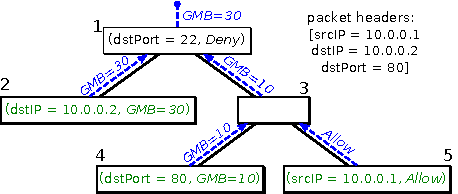
\includegraphics[width=0.7\textwidth]{figs/evaltree}
\caption{Evaluation of a single packet}
\label{f:evaltree}
\end{figure}


\vspace{0.5em}\noindent\textbf{Example:\space}
Figure~\ref{f:evaltree} depicts a simple policy tree
and illustrates how $\mathit{eval}$ produces an action, given the 
tree and indicated packet.
Each node contains its policy atoms, and atoms which match the packet are colored
green. The $\mathit{eval}$ function recursively produces an action from
each sub-tree; these actions are the labels on each node's outgoing edge.

In this example, the policy atoms at each leaf match the packet and produce
an action.
Node $3$ receives conflicting actions
from its children, which it resolves with its inter-sibling
conflict-resolution operator:
$\textbf{Reserve}(10)
+_S \textbf{Allow} = \textbf{Reserve}(10)$. Node $3$ has no policy atoms
itself, so it produces the $\textbf{0}$ action. Since $\textbf{0}$ is
the identity of all conflict-resolution operators,
  $\textbf{0} +_P \textbf{Reserve}(10) = \textbf{Reserve}(10)$ is the
resulting action from this sub-tree. 

Finally, Node 1 computes the aggregate action of its children:
$\textbf{Reserve}(30) +_S \textbf{Reserve}(10) = \textbf{Reserve}(\max(30,10))$.
Since Node 1's policy atoms do not match the packet,
the final action is
$\textbf{0} +_P \textbf{Reserve}(30) = \textbf{Reserve}(30)$.


\subsection{Compiling Policies}\label{s:lin}

The preceding section assumes that a central function,
$\mathit{eval}$, observes and directs all packets in the network.
Although $\mathit{eval}$ specifies the meaning of policy trees, this is not a
practical implementation. We now describe how to compile \treelang's
policy trees to run on commodity switches, which support simpler, linear
flow tables, to produce a practical implementation.

Our compiler works in two stages. First, we translate policy trees to
\emph{network flow tables}, which have a basic,
linear matching semantics. Second, we use
network flow tables to configure a distributed network of switches,
translating high-level actions such as $\textbf{GMB}(n)$ to low-level
operations on switches (\Cref{sec:NIB}).

\begin{figure}[t]

\begin{displaymath}
\begin{array}{lrcl}
\textrm{Network Flow Tables} & N & = & \langle \overrightarrow{M,A} \rangle
\end{array}
\end{displaymath}

\fbox{$\mathit{scan} : N \times K \rightarrow A$}

\medskip

\inference
{M_1\cap K = \emptyset \cdots M_{j-1} \cap K = \emptyset \qquad
 M_j\cap K \ne \emptyset }
{\mathit{scan}(\langle(M_1,A_1)\cdots(M_n,A_n)\rangle,K) = A_j}

\medskip

\inference
{M_1\cap K = \emptyset \cdots M_{n} \cap K = \emptyset}
{\mathit{scan}(\langle(M_1,A_1)\cdots(M_n,A_n)\rangle,K) = \textbf{0}}


\medskip

\fbox{$\mathit{lin}_D : D \rightarrow N$}
\begin{displaymath}
\begin{array}{l}
\mathit{lin}_D\left(+_D,\{M_1,A_1, \cdots, M_j,A_j \}\right) 
  = N_1 \\
\begin{array}{lllll}
\textrm{where} 
& N_1 = \mathit{union}(+_D,\langle M_1,A_1\rangle, N_2) \\
& \cdots \\
& N_j = \mathit{union}(+_D, \langle M_j,A_j\rangle, \langle\rangle)
\end{array}
\end{array}
\end{displaymath}

\fbox{$\mathit{lin}_T : T \rightarrow N$}
\begin{displaymath}
\begin{array}{l}
\mathit{lin}_T\left(+_P,+_S,D, \{T_1\cdots T_k\}\right)
  = \mathit{union}(+_P,\mathit{lin}_D(D), N_1) \\
\begin{array}{lllll}
\textrm{where} 
& N_1 = \mathit{union}(+_S, \mathit{lin}_T(T_1), N'_2) \\
& \cdots \\
& N_k = \mathit{union}(+_S,\mathit{lin}_T(T_k), \langle \rangle)
\end{array}
\end{array}
\end{displaymath}

\fbox{$\mathit{union},\mathit{inter} : (+) \times N \times N \rightarrow N$}
\begin{displaymath}
\begin{array}{l}
\mathit{union}((+),N_1,N_2) = \mathit{inter}((+),N_1,N_2) N_1 N_2 \\
\mathit{inter}((+),\langle\cdots(M_i,A_i)\cdots\rangle, \langle\cdots(M'_j,A'_j)\cdots\rangle) = \\
\qquad \langle\cdots(M_i \cap M'_j,A_i+A'_j))\cdots\rangle
\end{array}
\end{displaymath}

\caption{Network Flow Tables}
\label{f:intermediate}

\end{figure}

A network flow table ($N$) is a sequence of paired match rules
and actions. The $\mathit{scan}$ function, defined in
Figure~\ref{f:intermediate}, matches packets against network flow
tables and returns the action associated with the first matching rule. If
no rules match the packet, then $\mathit{scan}$ returns $\textbf{0}$.\footnote{The
  $\mathit{scan}$ function is derived from 
  NetCore~\cite{monsanto:popl12-netcore}.}

The matching semantics of network flow tables correspond to the
matching semantics of switch flow tables exposed by OpenFlow.  When a
packet matches a switch flow table, only one rule's action applies. If a
packet matches multiple rules, the switch selects the one with the
highest priority.  A rule's index in a network flow table corresponds
to a switch flow table priority, with index $0$ as the highest
priority. Since all rules have distinct indices, a naive
correspondence would give all rules distinct priorities. A more
compact one, which we use, maps a sequence of
non-overlapping network flow table rules to a single priority in a
switch flow table.

The $\mathit{lin}_T$ function is our compiler from policy trees to
network flow tables. It uses $\mathit{lin}_D$ as a helper to compile
policy tree nodes.  The $\mathit{lin}_D$ function translates policy
atoms to singleton network flow tables, and combines them with
$\mathit{union(+,N,N')}$.  $\mathit{Union}$ builds a network flow table that
matches packets in either $N$ or $N'$. Moreover, when a packet
matches both $N$ and $N'$, $\mathit{union}$ computes the intersection
using the $+$ conflict-resolution operator to combine
actions.

Similarly, $\mathit{lin}_T$ recursively builds network flow tables for
its subtrees, and calls $\mathit{lin}_D$ on its root node.  It applies
$\mathit{union}$ to combine the results, using $+_S$ and $+_P$ where
appropriate.


The functions in Figure~\ref{f:intermediate}, $\mathit{lin}_T$,
$\mathit{lin}_D$, $\mathit{union}$, and $\mathit{inter}$ require the
conflict-resolution operators to satisfy the following properties.
\begin{wftree}[Well-formed] 
$T$ is well-formed if:
\begin{itemize}

\item All conflict-resolution operators are associative, and

\item $\textbf{0}$ is the identity of all conflict-resolution operators.
\end{itemize}
\end{wftree}
Proving the compiler correct requires the following key lemma, which
states that all conflict-resolution operators distribute over $\mathit{scan}$.
\begin{unioncommute}
For all $+$, $N_1$, and $N_2$, where $\textbf{0}$ is the identity of $+$,
$\mathit{scan}(\mathit{union}(+,N_1,N_2)) = \mathit{scan}(N_1) +
\mathit{scan}(N_2)$.
\end{unioncommute}
With this, we prove the compiler correct.
\begin{compilercorrect}[Soundness]
For all well-formed policy trees, $T$ and packets, $P$, $\mathit{eval}(T, P) =
\mathit{scan}(\mathit{lin}_T(T), P)$.
\end{compilercorrect}
We mechanize all our definitions and proofs using the Coq proof
assistant~\cite{coq}.\footnote{The complete proof is available with \sys's source code: \url{http://github.com/brownsys/pane}} \qed

\subsection{Conflict-resolution Operators in \sys}
\label{sec:conflict-resolution-operators}


As discussed previously, HFTs resolve conflicts through the use of conflict resolution operators.
These operators take two conflicting requests as input, and return a single
resolved request. For example, a packet which matches policy atoms from \priv{Reserve}(10)
and \priv{Reserve}(30) may be resolved to the higher guaranteed bandwidth,
\priv{Reserve}(30), as occurs at Node 1 in Figure~\ref{f:evaltree}.

\begin{figure}[t]
\begin{small}
\fbox{$+_P : A \times A \rightarrow A$}
\begin{displaymath}
\begin{array}{lclcl}
\textbf{Deny} & +_P & \textbf{Allow} & = & \textbf{Allow} \\
\textbf{Allow} & +_P & \textbf{Allow} & = & \textbf{Allow} \\
A_P & +_P & \textbf{Deny} & = & \textbf{Deny} \\
\textbf{Deny} & +_P & \textbf{Reserve}(n) & = & \textbf{Reserve}(n) \\
\textbf{Reserve}(m) & +_P & \textbf{Reserve}(n) & = & \textbf{Reserve}(\max(m,n)) \\
\textbf{Reserve}(m) & +_P & \textbf{Allow} & = & \textbf{Reserve}(m) \\
\textbf{Allow} & +_P & \textbf{Reserve}(m) & = & \textbf{Reserve}(n) \\
\textbf{Deny} & +_P & \textbf{Ratelimit}(n) & = & \textbf{Ratelimit}(n) \\
\textbf{Ratelimit}(m) & +_P & \textbf{Ratelimit}(n) & = & \textbf{Ratelimit}(\min(m,n)) \\
\textbf{Ratelimit}(m) & +_P & \textbf{Allow} & = & \textbf{Ratelimit}(m) \\
\textbf{Allow} & +_P & \textbf{Ratelimit}(m) & = & \textbf{Ratelimit}(n) \\
\end{array}
\end{displaymath}

\fbox{$+_S : A \times A \rightarrow A$}
\begin{displaymath}
\begin{array}{lclcl}
\textbf{Deny} & +_S & A_2 & = & \textbf{Deny} \\
\textbf{Reserve}(m) & +_S & \textbf{Reserve}(n) & = & \textbf{Reserve}(\max(m,n)) \\
\textbf{Reserve}(m) & +_S & \textbf{Allow} & = & \textbf{Reserve}(m) \\
\textbf{Ratelimit}(m) & +_S & \textbf{Ratelimit}(n) & = & \textbf{Ratelimit}(\min(m,n)) \\
\textbf{Ratelimit}(m) & +_S & \textbf{Allow} & = & \textbf{Ratelimit}(m) \\
\end{array}
\end{displaymath}
\end{small}
{\small The $+_S$ operator is commutative. We only show representative cases.}

\caption{\sys's conflict-resolution operators}
\label{f:sysconflicts}

\end{figure}

The \treelang design allows for complex
conflict-resolution operators, and could support different operators at
each node in the tree.
However, for \sys we chose simple conflict-resolution operators in the
interest of user and administrator understanding.
Figure~\ref{f:sysconflicts} specifies \sys's conflict-resolution
operators.
\sys's parent-child operator ($+_P$) specifies a ``child
overrides parent'' policy for admission control. \sys's $+_S$ and $+_D$
operators are identical, and specify a ``\priv{Deny} overrides
\priv{Allow} policy'' between siblings.

These operators' simple design is heavily influenced by \sys's
first come-first serve approach to granting requests -- for example,
the operators do not consider the principal who made the request;
each request is treated equally within its hierarchical context.
However, by taking advantage of this design flexibility, operators
which resolve conflicts by using priorities could be introduced.
Because such an approach would lead to previously accepted requests
being preempted, the \sys controller would need to maintain a
connection to each principal to provide preemption notifications.
Avoiding this complexity is an additional benefit of \sys's current,
simple approach.

Finally, it is important to note that \sys's conflict-resolution operators
may drop previously realized hints to fulfill \emph{strict} requests,
detailed next, as needed.

\subsection{Strict vs Partial Fulfillment}
\label{sec:strict-partial}

We now return to \sys's \emph{strict} and \emph{partial} modes of
fulfillment, first introduced with the \priv{Allow} and \priv{Deny}
privileges. In each mode, a request is first authenticated against the
share tree, then, as shown in Figure~\ref{f:system}, \sys verifies the resulting policy tree can be
compiled to a valid network configuration.
After this verification, the two modes differ.

In strict mode, \sys ensures that a request's specified action
is the same as the action returned by HFT's \emph{eval}
function for all packets in the request's flowgroup -- that is, no
conflict resolution operator has changed the resulting action for
any matching packets.
More formally, when a request with match rule $M$ and action
$A$ is added to a policy tree, yielding tree $T$,
$\forall\ \mathrm{packets}\ K \in \{ K | M \cap K \ne \emptyset \}, \mathit{eval} (T, K) = A$.
If this condition does not hold, the request is rejected.
In partial mode, the request is not subject to this check, and may
even be relaxed -- for example, a request for 30 Mbps of guaranteed
bandwidth on a share with only 20 Mbps available will be relaxed
to a request for 20 Mbps. 

These modes are useful for three reasons. First, strict mode provides
the principal with a guarantee that the request will be implemented
in the network as specified. This is a limited form of change-impact
analysis: \emph{was the impact of my change on the network's configuration
what I expected? If not, cancel the request.} We will expand
\sys's ability to provide change-impact analysis in future work.

Second, partial mode improves support
for concurrent requests, as at least a relaxed form of a partial request will succeed.
Without this, a principal faces the risk of repeatedly crafting
strict requests based on the network state at time $t_0$, only to have
the request arrive at time $t_2 > t_0$ and conflict with a request
accepted at time $t_1$, where $t_2 > t_1 > t_0$.

Finally, partial mode's ability to relax a request is a useful convenience.
For example, if a principal has permissions which affect dozens of
specific TCP ports in the range 1000-2000, yet not all of them, partial
requests can be made for that range, and the requests would be relaxed to
just the specific ports, freeing the principal from needing to specify the
particular ports on each request.

Partial reservations, such as the 20 Mbps received of the 30 Mbps requested
in the example above, are particularly useful as
applications can use them to provide upper-bounds for transfer time. Although the
faster reservation may have been preferred, the slower one still provides
predictability to the end-user (and in either scenario, the actual bandwidth
received by the transfer may be even higher than the guaranteed minimum).
Such a use case is different from that for bandwidth hints; with hints, the
principal does not know how the information will be used, if at all.

\begin{comment}
Can discuss why partial reservations make sense -- operations such as a
data backup can get a guarantee from the network, which allows them to
provide a predictable experience for the user. however, they don't need to
get a guarantee as high as the one they requested. this is different from a
hint situation in which the network control-plane understands more about
the traffic, say, that it will be predictable (information it can feed to
something like Theo's MicroTE) or that it will be a large flow, so that the
controller can proactively split elephant flows across redundant links.
\end{comment}

\section{Compiler Complexity}
\label{sec:compiler-complexity}

To realize a policy tree in OpenFlow hardware, we have to compile it
to flow tables for each switch. We use a variation of
Hierarchical Flow Tables (HFT)~\cite{Ferguson:2012b}. A direct
implementation of the HFT algorithm produces flow tables of size
$O(2^n)$, where $n$ is the size of the policy tree. The earlier
algorithm is therefore useless on all but trivial policies.  However,
we make two changes that greatly reduce the complexity:
the modified algorithm yields flow tables
of size $O(n^2)$ in $O(n^2)$ time. This section is an overview of our
results. 

OpenFlow flow tables are simple linear
sequences of patterns and actions. A flow can match several,
overlapping policy atoms in a policy tree and trigger
conflict-resolution that combines their policies. However, in an
OpenFlow flow table, a flow will only trigger the action of the
highest-priority matching pattern.

For example, suppose the policy tree has two atoms with the following
flowgroups:
\[
\begin{array}{l}
\paneshare{X}{Y}{\texttt{tcp}}{\star}{\star} \\
\paneshare{\star}{\star}{\texttt{tcp}}{\star}{\texttt{80}}
\end{array}
\]
Suppose flows that match the first flowgroup -- all flows from $X$ to
$Y$ -- are waypointed through some switch, and that flows that match
the second flowgroup -- all HTTP requests -- are given some bandwidth
reservation.  These two flowgroups overlap, thus a flow may be (1)
waypointed with a reservation, (2) only waypointed, (3) only given a
reservation, or (4) not be affected by the policy.

An OpenFlow flow table that realizes the above two-atom policy tree must have
entries for all four cases.  The original algorithm~\cite{Ferguson:2012b}
generates all possible combinations given trees of size $n$ --- \ie flow tables
of size $O(2^n)$.

We make two changes to prune the generated flow table: (1) we remove
all rules that generate empty patterns and (2) we remove all rules
whose patterns are fully shadowed by higher-priority rules. The
earlier algorithm is recursive, and we prune after each recursive
call.  It is obvious that this simple pruning does not affect the
semantics of flow tables. However, a surprising result is that it
dramatically improves the complexity of the algorithm.

The intuition behind our proof is that for sufficiently large policy trees,
the intersections are guaranteed to produce
duplicate and empty patterns that get pruned. To see this,
note OpenFlow patterns have a bit-vector that determines which fields
are wildcards.  Suppose two patterns have identical wildcard bits and
we calculate their intersection:

First, if the two patterns are identical, then so is their
  intersection. Of these three identical patterns, two get pruned.
Second, if the two patterns are distinct, since their wildcards are
  identical, they exactly match some field differently. Thus, their
  intersection is empty and pruned.

If patterns have $h$ header fields, there are only $2^h$ unique
wildcard bit-vectors. Therefore, if a policy tree has more than $2^h$
policy atoms, it is assured that some intersections create empty or duplicate
patterns that are pruned.

Our full complexity analysis shows that when the
number of policy atoms, $n$, is larger than $2^h$, then the
compilation algorithm runs in $O(n^2)$ time and produces a flow table
of size $O(n^2)$. OpenFlow 1.0 patterns are $12$-tuple, and our current
policies
only use $5$ header fields. Therefore, on policies
with more than $2^5$ policy atoms, the algorithm is quadratic.

\tightparagraph{Updating Flow Tables}

It is not enough for \sys to generate flow tables quickly. It must
also propagate switch updates quickly, as the time required to update
the network affects the effective duration of requests.
The OpenFlow protocol only allows switches to be updated one rule at a
time.  A naive strategy is to first delete all old rules, and then
install new rules. In \sys, we implement a faster strategy: the
controller state stores the rules deployed on each switch; to install
new rules, it calculates a ``diff'' between the new and old
rules. These diffs are typically small, since rule-table updates occur
when a subset of policy atoms are realized or unrealized.


